\documentclass[submission,copyright,creativecommons]{eptcs}
\providecommand{\event}{PLACES 2020} % Name of the event you are submitting to
%\usepackage{breakurl}             % Not needed if you use pdflatex only.

\usepackage{wrapfig}
\usepackage{graphicx}
\usepackage{subcaption}
\usepackage{stmaryrd}
\usepackage[strings]{underscore}
\usepackage{color}
\definecolor{purple}{rgb}{0.65, 0.12, 0.82}
\definecolor{darkgray}{rgb}{.4,.4,.4}

\usepackage{listings}
\lstdefinelanguage{Scribble}{
  keywords={module, type, from, as, global,protocol, role, to, choice, at, or, do},
  keywordstyle=\color{blue}\bfseries,
  identifierstyle=\color{black},
  sensitive=false,
  comment=[l]{//},
  morecomment=[s]{/*}{*/},
  commentstyle=\color{darkgray}\ttfamily,
  stringstyle=\color{purple}\ttfamily,
  morestring=[b]',
  morestring=[b]"
}
\lstdefinelanguage{JavaScript}{
  keywords={typeof, new, true, false, catch, function, return, null, catch, switch, var, if, in, while, do, else, case, break, class, export, boolean, throw, implements, import, this, const, let, extends},
  keywordstyle=\color{blue}\bfseries,
%  ndkeywords={class, export, boolean, throw, implements, import, this},
%  ndkeywordstyle=\color{darkgray}\bfseries,
  identifierstyle=\color{black},
  sensitive=false,
  comment=[l]{//},
  morecomment=[s]{/*}{*/},
  commentstyle=\color{darkgray}\ttfamily,
  stringstyle=\color{purple}\ttfamily,
  morestring=[b]',
  morestring=[b]"
}
\lstset{
	basicstyle=\footnotesize\ttfamily,
	numbers=left,
	frame=single,
}
\usepackage{caption}

\newcommand{\sectionref}[1]{\textsection~\ref{#1}}

\title{Multiparty Session Type-safe Web Development in TypeScript}
\author{Anson Miu
\institute{Imperial College London}
\and
Francisco Ferreira
\institute{Imperial College London}
\and
Nobuko Yoshida
\institute{Imperial College London}
\and
Fangyi Zhou
\institute{Imperial College London}
}
\def\titlerunning{MPST-safe Web Development in TypeScript}
\def\authorrunning{A. Miu, F. Ferreira, N. Yoshida \& F. Zhou}
\begin{document}
\maketitle

\begin{abstract}
% Situation: webapps, interactive, JavaScript more powerful but remains a poor language for maintaing large applications

% Problem: hard to maintain/test
% New languages (like Dart and TypeScript)

% Solution: MPST for web development

This is a sentence in the abstract.
This is another sentence in the abstract.
This is yet another sentence in the abstract.
This is the final sentence in the abstract.

% Problem: similar to PureScript paper

% In this paper, we present...

% TypeScript
% - gradual type system, superset of JavaScript
% - we define how our approach achieves "gradual linearity" (can we define this?)
%Our work targets TypeScript - a superset of \dots

%We demonstrate the effectiveness of our approach through a web-based game of \textit{Noughts and Crosses} where communication is performed through WebSocket connections.

\end{abstract}

\section{Introduction}
% Situation: stateful communication over WebSocket and interactive web applications

Modern interactive web applications aim to provide a highly responsive user experience by minimising the communication latency between clients and servers. 
Whilst the HTTP request-response model is sufficient for retrieving static assets, applying the same stateless communication approach for interactive use cases (such as a multiplayer game) introduces undesirable performance overhead from having to frequently set up new connections for client-server interactions. 
Developers have since adopted other communication transport abstractions over HTTP connections such as the WebSockets protocol \cite{WebSocketRFC} to enjoy low-latency full-duplex client-server communication in their applications over a single persistent connection. 
Enabling more complex communication patterns caters for more interactive use cases (such as real-time multiplayer games), but introduces additional concerns to the developer with respect to implementation correctness.

% Example: naughts and crosses
Consider a classic turn-based board game of \textit{Noughts and Crosses} between two players. Both players are identified by either noughts or crosses respectively, and take turns to place a mark on an unoccupied cell of a 3-by-3 grid until one player wins (when their markers form one straight line on the board) or a stalemate is reached (when all cells are occupied).

Figure \ref{fig:tictactoe} illustrates a possible implementation of the game as an interactive real-time multiplayer web application. Both players are connected to the game server by bidirectional WebSocket connections and interact with the game from their web browser, which serve a \textit{single-page application} (SPA) of the game client. SPAs feature a single HTML page and dynamically renders content via JavaScript in the browser. Players take turns to make a move on the game board and the server implements the game logic to progress the game forward until a result (either a win/loss or draw) can be declared. 

Whilst WebSockets make this web-based implementation possible, it introduces the developer to a new family of communication errors, even for this simple game. In addition to the usual testing for game logic correctness, the developer needs to test against \textit{deadlocks} (e.g. both players waiting for each other to make a move at the same time) and \textit{communication mismatches} (e.g. player 1 sending a boolean to the game server instead of the board coordinates). The complexity of these errors, which correlate to the complexity of tests required against these errors, scale with the complexity of the communication patterns involved.

\textit{Multiparty Session Types} (MPST) \cite{MPST} provide a framework for formally specifying a structured communication pattern between concurrent processes and verifying implementations for correctness with respect to the communications aspect. By specifying the client-server interactions of our game as a protocol and verifying the implementations against the protocol for well-formedness, MPST theory guarantees well-formed implementations to be free from communication errors.

This MPST methodology has been applied to target applications written in both statically and dynamically typed languages in \cite{Hybrid2016, Python2017}, but do not apply to the event-driven paradigm of interactive web applications. A proposal that caters for web applications in \cite{PureScript2019} targets PureScript to maximise the static guarantees it can provide, but the strong type system make it difficult to extract common code and the functional paradigm is arguably unidiomatic relative to mainstream web development in JavaScript, which limits developer productivity. JavaScript began as the language of the web browser, but a shallow learning curve, an ever-growing ecosystem of libraries and frameworks (such as React.js for writing SPAs) and a successful server-side single-threaded event loop implementation in \textit{Node.js} has propelled it as the de-facto choice for full-stack web application development in a single language. 

Whilst the proposal in \cite{Python2017} could be adapted to verify interactive web applications written in JavaScript, the emergence of Microsoft's TypeScript \cite{TypeScript} with a gradual type system motivates the need for a MPST-based workflow for verifying full-stack TypeScript web applications, such that it is flexible with respect to idiomatic practices and frameworks to be useful in industry whilst also leveraging the language features to maximise the static guarantees it is able to provide. Such a workflow would ultimately decrease the overhead for incorporating MPST into mainstream web development, which reduces development time by programmatically verifying implementations for communication correctness.

\paragraph{Contributions}
This paper presents a workflow for developing type-safe interactive SPAs motivated by the MPST framework: \textbf{(1)} An endpoint API code generation workflow targeting TypeScript-based web applications for multiparty sessions; \textbf{(2)} An encoding of session types in server-side TypeScript that enforces static linearity; and \textbf{(3)} An encoding of session types in browser-side TypeScript using the React framework that guarantees affine usage of communication channels.

Figure \ref{fig:workflow} illustrates our proposed development workflow: we extend the Scribble framework (\sectionref{section:scribble}) and generate TypeScript endpoints for server-side (\sectionref{section:server}) and browser-side (\sectionref{section:browser}) targets. We will use the \textit{Noughts and Crosses} game as our running example in the rest of the paper and show how our approach is a practical compromise that combines benefits from static session typing and being compatible with common libraries and idiomatic JavaScript practices (\sectionref{section:example}).

\section{The Scribble Framework}
\label{section:scribble}
Development begins by specifying the permitted communications between participants as a \textit{global protocol} in Scribble, a MPST-based framework introduced in \cite{Scribble} which features a protocol specification language and code generation toolchain. This means that a protocol specified in Scribble maps to some \textit{global type} in multiparty session type theory \cite{MPST}.

We specify the \textit{Noughts and Crosses} game as a Scribble protocol in Listing \ref{lst:game} and explain the syntax of the language through this example. 
Scribble protocols are organised into \textit{modules}: line 1 declares the name of the module. Line 2 declares a message type to be used as payload types in the global protocol: this would correspond to an \texttt{import \{ Coordinate as Point \} from './Types'} statement in TypeScript, where the developer provides the definition of the \texttt{Coordinate} interface under a \texttt{Types.ts} file.
Line 4 declares the name of the global protocol (\texttt{Game}) and specifies the participants involved in the protocol as \textit{roles}; the protocol body is defined by lines 5-16.
A message passing statement from a sender (e.g. \texttt{P1}) to a receiver (e.g. \texttt{Svr}) require a \textit{label identifier} followed by a list of \textit{payload types} in parentheses (e.g. \texttt{Pos(Point) from P1 to Svr} on line 5).
Semicolons denote continuations for message passing statement in the same way that they express sequential statement execution in programming languages such as Java.

\begin{figure}[!h]
\begin{lstlisting}[
	language=Scribble
]
module NoughtsAndCrosses;
type <typescript> "Coordinate" from "./Types" as Point;	// Position on board

global protocol Game(role Svr, role P1, role P2) {
  Pos(Point) from P1 to Svr;
  choice at Svr {
    Lose(Point) from Svr to P2;
    Win(Point) from Svr to P1;
  } or {
    Draw(Point) from Svr to P2;
    Draw(Point) from Svr to P1;
  } or {
    Update(Point) from Svr to P2;
    Update(Point) from Svr to P1;
    do Game(Svr, P2, P1);
  }
}
\end{lstlisting}
\captionof{lstlisting}{Main body of the \textit{Noughts and Crosses} protocol.}
\label{lst:game}
\end{figure}

The \texttt{Game} protocol involves three roles: the server (\texttt{Svr}) and two players (\texttt{P1} and \texttt{P2}). First, \texttt{P1} makes a move by sending a coordinate to place the marker on the game board to \texttt{Svr}. Upon receiving the \texttt{Pos} message, \texttt{Svr} will implement the game logic to decide the outcome of \texttt{P1}'s move and communicate with \texttt{P2} accordingly. We express this as a \texttt{choice} statement (lines 6-15), where \texttt{Svr} decides whether \texttt{P1}'s move resulted in a loss for \texttt{P2} (lines 7-8), stalemate (lines 10-11) or an unfinished game (lines 13-15).

If \texttt{P1} performed a winning move (i.e. the latest coordinate resulted in three-in-a-row for \texttt{P1}), then \texttt{Svr} sends a \texttt{Lose} message to \texttt{P2} and a \texttt{Win} message to \texttt{P1} with the coordinates of the latest move. These coordinates are sent to allow the applications running in the browser for both players to update their version of the game state respectively; how they choose to render this on the DOM is up to their implementation, independent of the protocol. Similar message passing actions are sent in the case of a draw, just with updated labels for \texttt{Draw}. 

Otherwise, the game has not ended, so \texttt{Svr} updates both players with the coordinates of the latest move by sending an \texttt{Update} message, and the game proceeds to allow \texttt{P2} to make a move. We express this as a recursive call to the \texttt{Game} protocol using a \texttt{do} statement: note that we swap the role parameters \texttt{P2} and \texttt{P1} to express the turn-taking semantics of the game. In short, the global protocol describes \texttt{P1} and \texttt{P2} taking turns until \texttt{Svr} declares a winner/loser or draw.

We leverage the Scribble toolchain to check for protocol well-formedness. This directly corresponds to the multiparty session type theory of verifying valid local type \textit{projections} for all participants of a global type. The implementation of this validation by the toolchain follow from the algorithmic projection procedures defined in \cite{MPST}. We obtain \textit{endpoint protocols} for each role in a well-formed global protocol. An endpoint protocol only preserves the interactions defined by the global protocol in which the target role is involved. For example, the endpoint protocol for \texttt{P1} will not include the exchange of messages between \texttt{Svr} and \texttt{P2}. An endpoint protocol corresponds to an equivalent \textit{Endpoint Finite State Machine} (EFSM) in the Scribble toolchain. We adopt the formalism of EFSMs in \cite{Hybrid2016}, and use the EFSMs as a basis for API generation.


\section{Encoding Session Types in TypeScript}
% Design choices

Developers can validate the communication aspects of their implementation against their EFSM to verify protocol conformance. Our approach integrates the EFSM into the development workflow by encoding session types as TypeScript types. We appreciate the inherent differences in development considerations between front- and back-end web development: business logic tends to initiate communication in the back-end, whilst communication in the front-end is mostly driven by user interactions with the browser. This motivates our design choice of generating different session types encodings for the target application on the server (\sectionref{section:server}) and in the browser (\sectionref{section:browser}).

\subsection{Server-side API generation}
\label{section:server}

\begin{wrapfigure}{r}{0.5\textwidth}
  \begin{center}
    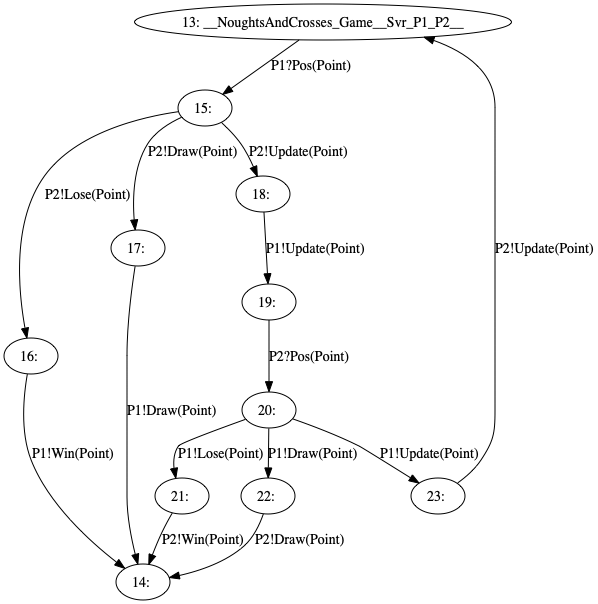
\includegraphics[width=0.48\textwidth]{figures/efsm_svr.png}
  \end{center}

  \captionof{figure}{EFSM for \texttt{Svr} in \textit{Noughts and Crosses}.}
  \label{fig:efsmsvr}
\end{wrapfigure}

We will refer to the \texttt{Svr} EFSM (fig.~\ref{fig:efsmsvr}) as a running example in this section. For server-side targets, we encode EFSM states as TypeScript types depending on the type of state. We adopt the EFSM definition presented in \cite{Hybrid2016} to consider receive and send states separately. We assign each TypeScript encoding its state identifier from the EFSM as its type alias, thus providing syntactic sugar when referring to the successor state in the TypeScript encoding of the current state. For any state $S$ in the EFSM, we refer to the TypeScript type alias of its encoding as $\llbracket S \rrbracket$. 

We make a key design decision \textit{not} to expose communication channels in the TypeScript session type encodings to provide linearity guarantees (\sectionref{section:serverlinear}). Our encodings sufficiently exposes seams for the developer to inject their business logic, whilst the generated session API (\sectionref{section:serversessionapi}) handles the sending and receiving of messages; as a result, the encodings do not concern with the role involved in the send/receive action. We outline the encodings below using examples from the \textit{Noughts and Crosses} game server (listing \ref{lst:svr}).

\paragraph{Branching state} We consider a receive state as a unary branching state for conciseness. A branching state is encoded as an \textit{object literal} \cite{TypeScriptSpec}, with each branch corresponding to a member field. A branch expecting to receive a message labelled $\texttt{label}_i$ carrying payload of type $\texttt{T}_i$ with successor state $S_i$ is encoded as an \textit{member field} named $\texttt{label}_i$ of function type \texttt{(payload:$\texttt{T}_i$) => $\llbracket S_i \rrbracket$}. The developer implements a branching operation by passing callbacks for each branch, parameterised by the expected message payload type for that branch.

\paragraph{Selection state} We consider a send state as a unary selection state for conciseness. A selection state is encoded as a \textit{union type} \cite{TypeScriptSpec} of internal choice encodings: each internal choice sending a message labelled $\texttt{label}_i$ carrying payload of type $\texttt{T}_i$ with successor state $S_i$ is encoded as a \textit{tuple type} of \texttt{[Labels.label$_i$, T$_i$, $\llbracket S_i \rrbracket$]}. The developer implements a selection operation by passing the selected label and payload to send in the message. We generate a \textit{string enum} (named \texttt{Labels}) wrapping the labels in the protocol, hence the enum member access in the first element of the tuple type.

\begin{figure}[!h]
\begin{lstlisting}[language=JavaScript, title=\texttt{./NoughtsAndCrosses/Game.ts}]
import { Coordinate as Point } from "./Types";
import { Labels } from "./Constants";

export type S13 = { Pos: (payload: Point) => S15 }
export type S15 = [Labels.Lose, Point, S16]
		| [Labels.Draw, Point, S17]
		| [Labels.Update, Point, S18]
\end{lstlisting}  
\captionof{lstlisting}{Example encodings from \textit{Noughts and Crosses} \texttt{Svr} EFSM.}
\label{lst:svr}
\end{figure}

\subsubsection{Session Runtime and Protocol API}
\label{section:serversessionapi}

Our session runtime performs communication in a way that conforms to the protocol specification. The runtime listens to message (receive) events on the communication channel, invokes the corresponding callback to obtain the value to send next, and performs the send.

The \textit{Protocol API} is a class that interfaces between the session runtime and the user implementation of the EFSM state encodings. Upon construction, the Protocol class waits for all client roles to connect via WebSocket, then proceeds to the initial state of the EFSM and performs state transitions depending on the permitted communication patterns from the EFSM. The Protocol class constructor requires the WebSocket server and the following handlers:

\paragraph{Initial state} When all roles have joined the session, the Protocol class needs to know what to do in the initial state to start communication, be it sending a message to a client or offering branches to a client. For the \textit{Noughts and Crosses} game server, this would be a callback to handle the receipt of the \texttt{Pos(Point)} message from \texttt{P1}.

\paragraph{Receive handlers for each role} The runtime needs to bind a message event listener to the WebSocket between the server and each (client) role, and needs to know how to handle the incoming messages. For each role, the user is required to pass callbacks that encode the receive states for that role. The type alias for such a handler is the \textit{intersection type} \cite{TypeScriptSpec} of all receive states concerning that role. Considering a hypothetical web-service providing addition and square root functionality to a client role \texttt{C}, if \texttt{S1} is a state expecting to receive \texttt{Add(int, int)} from \texttt{C} and \texttt{S4} is a state expecting to receive \texttt{Sqrt(int)} from \texttt{C}, we define \texttt{type Receive_C = S1 \& S4} as the receive handler type alias and the user needs to pass some value of \texttt{Receive_C} when instantiating the session through the Protocol API. 

\subsubsection{Linear channel usage}
\label{section:serverlinear}
Our callback-oriented design for server-side API generation provides guarantees on state channel linearity by preventing the two properties detailed below. Here, channel linearity is guaranteed based on the correctness of our library design and session runtime implementation, which means a faulty implementation could violate this, but is up to the library author to verify once rather than the end user.

\paragraph{Repeat use} By adopting a callback-oriented design for server-side API generation, channels are not directly accessed by the programmer which makes \textit{reuse} impossible; only the Protocol API is exposed but channel operations are concealed in a private class. Consider the \textit{Noughts and Crosses} server endpoint: the programmer must pass a callback that handles the receipt of a \texttt{Pos(Point)} message and returns either a \texttt{Lose(Point)}, \texttt{Draw(Point)} or \texttt{Update(Point)} message with the appropriate continuation. Upon receiving the \texttt{Pos(Point)} message from a player, our lightweight runtime invokes the callback to get \texttt{Svr}'s choice from the return value, and perform the appropriate send. This is transparent to the programmer and it is impossible for the programmer to send or receive messages more than once, by design.

\paragraph{Unused} The initial state must be supplied to the Protocol API constructor in order to instantiate the session; this initial state is defined in terms of the successor states, which in turn has references to its successors and so forth. This encoding approach will cover the terminal state (if it exists in the EFSM, as \cite{Hybrid2016} notes that an EFSM contains at most one terminal state), and the session runtime guarantees this terminal state, if it exists, will be reached by construction. 

\subsection{Browser-side API generation}
\label{section:browser}

\begin{wrapfigure}{r}{0.5\textwidth}
  \begin{center}
    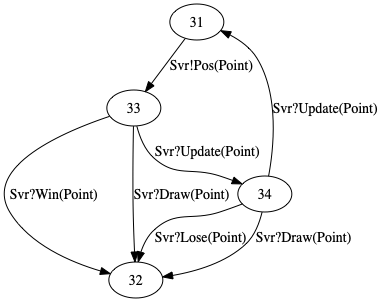
\includegraphics[width=0.48\textwidth]{figures/efsm_p1.png}
  \end{center}

  \captionof{figure}{EFSM for \texttt{P1} in \textit{Noughts and Crosses}.}
  \label{fig:efsmp1}
\end{wrapfigure}

We will refer to the \texttt{P1} EFSM (figure \ref{fig:efsmp1}) as a running example in this section. Preserving behavioural typing and channel linearity are known to be challenging for browser-side applications due to the event-driven nature of user interaction: in the case of \textit{Noughts and Crosses}, once the user makes a move by clicking on a cell on the game board, this click event must be deactivated until the user's next turn, otherwise the user can click again and violate channel linearity. Our design goal is to enforce this statically through the APIs we generate. For browser-side targets, we extend the approach presented in \cite{MVU2019} on \textit{multiple model types} motivated by the \textit{Model-View-Update} (MVU) architecture. Each state in the EFSM is a model type and uniquely defines a \textit{view function}, set of \textit{messages} and \textit{update function}: the view function defines what to render to the DOM, the set of messages define the possible (IO) actions available at that state, and the update function defines which successor state to transition to, given some supported IO action at this state.

\subsubsection{The React Framework}
Rather than using the LINKS web programming language from \cite{MVU2019}, we apply the multiple model types approach to the React framework \cite{React} developed by Facebook. React is widely used in industry to create scalable single-page TypeScript applications, and we intend for our proposed workflow to be beneficial in an industrial context. We introduce the key features of the framework below.

\paragraph{Components} A component is a reusable UI element which contains its own markup and logic. Components implement a \texttt{render()} function which returns a React element, the smallest building blocks of a React application. Components can keep \textit{state} and the \texttt{render()} function is invoked upon a change of state. A simple counter can be implemented as a component, with the count stored as state, a button which increments the count when clicked and a \texttt{div} that renders the current count. Components can also render other components, which gives rise to a parent/child relationship between components. Parents can pass data to children as \textit{props}, so the counter component could render a  child component \texttt{<StyledDiv count=\{this.state.count\} />} and propagate the count in the state to the child to reuse an existing UI element.

\paragraph{Virtual DOM} React components are rendered on a logical abstraction of the DOM, which in turn performs a \texttt{diff} on the current browser DOM and patches the delta accordingly. This allows the programmer to directly specify what should be rendered without having to worry about which elements to append or remove from the browser DOM.


\subsubsection{Model types in React}
We leverage React to express the model types approach in \cite{MVU2019} rather than the \textit{Model-View-Controller} (MVC) architecture it was intended for. 

\paragraph{State} \dots

\paragraph{Model transitions - message receive} \dots

\paragraph{Model transitions - message send} \dots

\subsubsection{Session instantiation}

\dots

% State = React component
% Send transitions = model transition factory
% Receive transitions = handled by 
% Protocol component = handle joining and rendering of correct EFSM component

\subsubsection{Affine channel usage}
A limitation of our browser-side session type encoding is only being able to guarantee that channel resources are used \textit{at most once} as supposed to \textit{exactly once}.

\paragraph{Repeat use} Communication channels are not exposed to the programmer so multiple sends are impossible. This does not restrict the programmer from binding the send action to exactly one UI event: for the \textit{Noughts and Crosses} game, we bind the \texttt{Pos(Point)} send action to each unoccupied cell on the game board, but the generated runtime ensures that, once an event bound to the send action is triggered, the send is only performed once and the successor state is rendered on the DOM to prevent multiple sends initiated by the user.

\paragraph{Unused} Our approach \textit{does not} statically detect whether all transitions in a certain state are bound to some UI event. This means that it is possible for an implementation to \textit{not} handle transitions to a terminal state but still type-check, so we cannot prevent unused states. Consider a hypothetical protocol where, in the current state, sending \texttt{Quit()} to some server role \texttt{S} transitions to the terminal state: \dots

\section{Case Study}
\label{section:example}

\begin{figure}
\begin{lstlisting}[language=JavaScript, tabsize=4, title=\texttt{./app.ts}]
const handleP1Move: Receive_P1 = (move: Point) => {
	// User-implemented logic
	board.P1(move)
	if (board.won()) { return [Labels.Lose, move, move] }
	else if (board.draw()) { return [Labels.Draw, move, move] }
	else { return [Labels.Draw, move, handleP2Move] } 
}

const handleP2Move: Receive_P2 = ...

// Instantiate session
new NoughtsAndCrosses.Svr(webSocketServer, handleP1Move, handleP2Move)
\end{lstlisting}  
\captionof{lstlisting}{Example fragment of \textit{Noughts and Crosses} \texttt{Svr} implementation.}
\label{lst:svrprotocol}
\end{figure}

We apply our framework to implement a web-based implementation of the \textit{Noughts and Crosses} running example in TypeScript; the interested reader can find the full implementation in \cite{NoughtsAndCrosses}. In addition to showing the multiparty session type safety achieved by our generated APIs, we also show that our library design welcomes idiomatic JavaScript practices in the user implementation and is interoperable with common front- and back-end frameworks.
 
\subsection{Game server}
\label{section:exampleserver}
% TicTacToe example - backend

We set up the WebSocket server inside an Express.js \cite{ExpressJS} application on top of a Node.js \cite{NodeJS} runtime. We define our own game logic in a \texttt{Board} class to keep track of the game state and expose methods to query the result. This custom logic is integrated into our 
\texttt{Receive\_P1} and \texttt{Receive\_P2} handlers (listing \ref{lst:svrprotocol}) are defined using 

%\dots encapsulate our custom game logic in a class 



% Note: no state space explosion, allows for reusability

\subsection{Game clients}
% TicTacToe example - frontend

\paragraph{Implement states} \dots

\paragraph{Register states} \dots

\begin{figure}[!h]
\begin{lstlisting}[language=JavaScript, tabsize=4]
export class MakeMove extends S31 {
	render() {
		...
		{board.map((row, x) => (
			board.map((col, y) => {
				const SelectPoint = this.props.Pos('click', event => {
					event.preventDefault()
					return { x, y }
				}
				return <SelectPoint><td>.</td></SelectPoint>
			}
		)}
		...
	}
}
\end{lstlisting}  
\captionof{lstlisting}{Example fragment of \textit{Noughts and Crosses} \texttt{P1} implementation.}
\label{lst:clientapp}
\end{figure}

For the sake of sharing the same game client implementation for both players, \cite{NoughtsAndCrosses} uses \textit{higher-order components} (HOC) to build the correct state implementations depending on which player the user chooses to be. 

\section{Related Works}
%\paragraph{Languages with native session type support} \dots
% New languages written  (e.g. ATS)
%	- addresses the challenge of resource linearity with a liner type system
%	- problem with webdev: not compatible with libraries, technologies, flexibility of JavaScript (ultimately the language of the browser)

\paragraph{Endpoint API generation} \dots
% API generation
% - original Python implementation, generating monitors (Rumi's paper)
%	- Gradual type system lets us do better than just dynamic runtime checks
%	- could do the same approach with generating JavaScript monitors, but we have TS and Dart and can leverage more powerful type systems to do more static/compiler checks

% - Java (hybrid approach)
%	- leverage strongly typed system for static behavioural typing
%	- minimse dupliction by defining states in terms of IO interfaces (same IO state with different successor can still share code)
%	- runtime linearity checks

\paragraph{Session types in web development} \dots
% Session types in web development
% - purescript looking at the whole workflow
	% - problem: PureScript isn't as prevalent
% - simon fowler paper on MVU targeting linearity for frontend GUI 

\paragraph{Typestate programming} \dots
% Typestates (Mungo)
% - the React components we generate is essentially behaving like typestates of the role, where 
% each role has its set of permitted actions.

\section{Conclusion and Future Works}
We have presented a MPST-based framework for developing full-stack interactive TypeScript applications with WebSocket communications that conform to a protocol.

Future works include \dots

% Future work
% - generalise to encode protocols as typestates (e.g. Mungo example)
% - WebRTC for full MPST (since current limitation is w.r.t. MPST protocols with 1-server many-client roles


%\section{Introduction}
%% Emergence of interactive JavaScript-intensive applications that maintain continuous stateful
%
%The optional arguments of {\tt $\backslash$documentclass$\{$eptcs$\}$} are
%\begin{itemize}
%\item at most one of
%{\tt adraft},
%{\tt submission} or
%{\tt preliminary},
%\item at most one of {\tt publicdomain} or {\tt copyright},
%\item and optionally {\tt creativecommons},
%  \begin{itemize}
%  \item possibly augmented with
%    \begin{itemize}
%    \item {\tt noderivs}
%    \item or {\tt sharealike},
%    \end{itemize}
%  \item and possibly augmented with {\tt noncommercial}.
%  \end{itemize}
%\end{itemize}
%We use {\tt adraft} rather than {\tt draft} so as not to confuse hyperref.
%The style-file option {\tt submission} is for papers that are
%submitted to {\tt $\backslash$event}, where the value of the latter is
%to be filled in in line 2 of the tex-file. Use {\tt preliminary} only
%for papers that are accepted but not yet published. The final version
%of your paper that is to be uploaded at the EPTCS website should have
%none of these style-file options.
%
%By means of the style-file option
%\href{http://creativecommons.org/about/license/}{creativecommons}
%authors equip their paper with a Creative Commons license that allows
%everyone to copy, distribute, display, and perform their copyrighted
%work and derivative works based upon it, but only if they give credit
%the way you request. By invoking the additional style-file option {\tt
%noderivs} you let others copy, distribute, display, and perform only
%verbatim copies of your work, but not derivative works based upon
%it. Alternatively, the {\tt sharealike} option allows others to
%distribute derivative works only under a license identical to the
%license that governs your work. Finally, you can invoke the option
%{\tt noncommercial} that let others copy, distribute, display, and
%perform your work and derivative works based upon it for
%noncommercial purposes only.
%
%Authors' (multiple) affiliations and emails use the commands
%{\tt $\backslash$institute} and {\tt $\backslash$email}.
%Both are optional.
%Authors should moreover supply
%{\tt $\backslash$titlerunning} and {\tt $\backslash$authorrunning},
%and in case the copyrightholders are not the authors also
%{\tt $\backslash$copyrightholders}.
%As illustrated above, heuristic solutions may be called for to share
%affiliations. Authors may apply their own creativity here.
%
%Exactly 46 lines fit on a page.
%The rest is like any normal {\LaTeX} article.
%We will spare you the details.
%The rest is like any normal {\LaTeX} article.
%We will spare you the details.\\
%The rest is like any normal {\LaTeX} article.
%We will spare you the details.\\
%The rest is like any normal {\LaTeX} article.
%We will spare you the details.\\
%The rest is like any normal {\LaTeX} article.
%We will spare you the details.\\
%The rest is like any normal {\LaTeX} article.
%We will spare you the details.\hfill6\\
%The rest is like any normal {\LaTeX} article.
%We will spare you the details.\\
%The rest is like any normal {\LaTeX} article.
%We will spare you the details.\\
%The rest is like any normal {\LaTeX} article.
%We will spare you the details.\\
%The rest is like any normal {\LaTeX} article.
%We will spare you the details.\\
%The rest is like any normal {\LaTeX} article.
%We will spare you the details.\hfill11\\
%The rest is like any normal {\LaTeX} article.
%We will spare you the details.\\
%The rest is like any normal {\LaTeX} article.
%We will spare you the details.
%
%Here starts a new paragraph. The rest is like any normal {\LaTeX} article.
%We will spare you the details.
%The rest is like any normal {\LaTeX} article.
%We will spare you the details.\\
%The rest is like any normal {\LaTeX} article.
%We will spare you the details.\hfill16\\
%The rest is like any normal {\LaTeX} article.
%We will spare you the details.\\
%The rest is like any normal {\LaTeX} article.
%We will spare you the details.\\
%The rest is like any normal {\LaTeX} article.
%We will spare you the details.\\
%The rest is like any normal {\LaTeX} article.
%We will spare you the details.\\
%The rest is like any normal {\LaTeX} article.
%We will spare you the details.\hfill21\\
%The rest is like any normal {\LaTeX} article.
%We will spare you the details.\\
%The rest is like any normal {\LaTeX} article.
%We will spare you the details.\\
%The rest is like any normal {\LaTeX} article.
%We will spare you the details.\\
%The rest is like any normal {\LaTeX} article.
%We will spare you the details.\\
%The rest is like any normal {\LaTeX} article.
%We will spare you the details.\hfill26\\
%The rest is like any normal {\LaTeX} article.
%We will spare you the details.\\
%The rest is like any normal {\LaTeX} article.
%We will spare you the details.\\
%The rest is like any normal {\LaTeX} article.
%We will spare you the details.\\
%The rest is like any normal {\LaTeX} article.
%We will spare you the details.\\
%The rest is like any normal {\LaTeX} article.
%We will spare you the details.\hfill31\\
%The rest is like any normal {\LaTeX} article.
%We will spare you the details.\\
%The rest is like any normal {\LaTeX} article.
%We will spare you the details.\\
%The rest is like any normal {\LaTeX} article.
%We will spare you the details.\\
%The rest is like any normal {\LaTeX} article.
%We will spare you the details.\\
%The rest is like any normal {\LaTeX} article.
%We will spare you the details.\hfill36\\
%The rest is like any normal {\LaTeX} article.
%We will spare you the details.\\
%The rest is like any normal {\LaTeX} article.
%We will spare you the details.\\
%The rest is like any normal {\LaTeX} article.
%We will spare you the details.\\
%The rest is like any normal {\LaTeX} article.
%We will spare you the details.\\
%The rest is like any normal {\LaTeX} article.
%We will spare you the details.\hfill41\\
%The rest is like any normal {\LaTeX} article.
%We will spare you the details.\\
%The rest is like any normal {\LaTeX} article.
%We will spare you the details.\\
%The rest is like any normal {\LaTeX} article.
%We will spare you the details.\\
%The rest is like any normal {\LaTeX} article.
%We will spare you the details.\\
%The rest is like any normal {\LaTeX} article.
%We will spare you the details.\hfill46\\
%The rest is like any normal {\LaTeX} article.
%We will spare you the details.
%The rest is like any normal {\LaTeX} article.
%We will spare you the details.
%The rest is like any normal {\LaTeX} article.
%We will spare you the details.
%The rest is like any normal {\LaTeX} article.
%We will spare you the details.
%The rest is like any normal {\LaTeX} article.
%We will spare you the details.
%The rest is like any normal {\LaTeX} article.
%We will spare you the details.
%The rest is like any normal {\LaTeX} article.
%We will spare you the details.
%The rest is like any normal {\LaTeX} article.
%We will spare you the details.
%The rest is like any normal {\LaTeX} article.
%We will spare you the details.
%The rest is like any normal {\LaTeX} article.
%We will spare you the details.
%The rest is like any normal {\LaTeX} article.
%We will spare you the details.
%The rest is like any normal {\LaTeX} article.
%We will spare you the details.
%The rest is like any normal {\LaTeX} article.
%We will spare you the details.
%The rest is like any normal {\LaTeX} article.
%We will spare you the details.
%The rest is like any normal {\LaTeX} article.
%We will spare you the details.
%The rest is like any normal {\LaTeX} article.
%We will spare you the details.
%The rest is like any normal {\LaTeX} article.
%We will spare you the details.
%
%\section{Prefaces}
%
%Volume editors may create prefaces using this very template,
%with {\tt $\backslash$title$\{$Preface$\}$} and {\tt $\backslash$author$\{\}$}.
%
%\section{Bibliography}
%
%We request that you use
%\href{http://www.cse.unsw.edu.au/~rvg/EPTCS/eptcs.bst}
%{\tt $\backslash$bibliographystyle$\{$eptcs$\}$}
%\cite{bibliographystylewebpage}. Compared to the original {\LaTeX}
%{\tt $\backslash$biblio\-graphystyle$\{$plain$\}$},
%it ignores the field {\tt month}, and uses the extra
%bibtex fields {\tt eid}, {\tt doi}, {\tt ee} and {\tt url}.
%The first is for electronic identifiers (typically the number $n$
%indicating the $n^{\rm th}$ paper in an issue) of papers in electronic
%journals that do not use page numbers. The other three are to refer,
%with life links, to electronic incarnations of the paper.
%
%Almost all publishers use digital object identifiers (DOIs) as a
%persistent way to locate electronic publications. Prefixing the DOI of
%any paper with {\tt http://dx.doi.org/} yields a URI that resolves to the
%current location (URL) of the response page\footnote{Nowadays, papers
%  that are published electronically tend
%  to have a \emph{response page} that lists the title, authors and
%  abstract of the paper, and links to the actual manifestations of
%  the paper (e.g.\ as {\tt dvi}- or {\tt pdf}-file). Sometimes
%  publishers charge money to access the paper itself, but the response
%  page is always freely available.}
%of that paper. When the location of the response page changes (for
%instance through a merge of publishers), the DOI of the paper remains
%the same and (through an update by the publisher) the corresponding
%URI will then resolve to the new location. For that reason a reference
%ought to contain the DOI of a paper, with a life link to corresponding
%URI, rather than a direct reference or link to the current URL of
%publisher's response page. This is the r\^ole of the bibtex field {\tt doi}.
%DOIs of papers can often be found through
%\url{http://www.crossref.org/guestquery};\footnote{For papers that will appear
%  in EPTCS and use \href{http://www.cse.unsw.edu.au/~rvg/EPTCS/eptcs.bst}
%  {\tt $\backslash$bibliographystyle$\{$eptcs$\}$} there is no need to
%  find DOIs on this website, as EPTCS will look them up for you
%  automatically upon submission of a first version of your paper;
%  these DOIs can then be incorporated in the final version, together
%  with the remaining DOIs that need to found at DBLP or publisher's webpages.}
%the second method {\it Search on article title}, only using the {\bf
%surname} of the first-listed author, works best.  
%Other places to find DOIs are DBLP and the response pages for cited
%papers (maintained by their publishers).
%{\bf EPTCS requires the inclusion of a DOI in each cited paper, when available.}
%
%Often an official publication is only available against payment, but
%as a courtesy to readers that do not wish to pay, the authors also
%make the paper available free of charge at a repository such as
%\url{arXiv.org}. In such a case it is recommended to also refer and
%link to the URL of the response page of the paper in such a
%repository.  This can be done using the bibtex fields {\tt ee} or {\tt
%url}, which are treated as synonyms.  These fields should not be used
%to duplicate information that is already provided through the DOI of
%the paper.
%You can find archival-quality URL's for most recently published papers
%in DBLP---they are in the bibtex-field {\tt ee}. In fact, it is often
%useful to check your references against DBLP records anyway, or just find
%them there in the first place.
%
%When using {\LaTeX} rather than {\tt pdflatex} to typeset your paper, by
%default no linebreaking within long URLs is allowed. This leads often
%to very ugly output, that moreover is different from the output
%generated when using {\tt pdflatex}. This problem is repaired when
%invoking \href{http://www.cse.unsw.edu.au/~rvg/EPTCS/breakurl.sty}
%{\tt $\backslash$usepackage$\{$breakurl$\}$}: it allows linebreaking
%within links and yield the same output as obtained by default with
%{\tt pdflatex}. 
%When invoking {\tt pdflatex}, the package {\tt breakurl} is ignored.
%
\nocite{*}
\bibliographystyle{eptcs}
\bibliography{generic}
\end{document}
